\documentclass[aspectratio=169]{beamer}
\usepackage{../../LaTex/simplemetropolis} % Load your custom style
% % Input encoding.
\usepackage[utf8]{inputenc} % For accents in spanish: transforms "á" into "\'a"
\usepackage[T1]{fontenc} % Output encoding. Use to avoid silly problems on the output.
                         % See: http://tex.stackexchange.com/questions/664/why-should-i-use-usepackaget1fontenc
\usepackage{lmodern} % Latin Modern fonts have broader support
% AMS packages
\usepackage{amsmath}
\usepackage{amsfonts}
\usepackage{amssymb}
\usepackage{amsthm}
\usepackage{bbm}
% Other maths packages
\usepackage{mathtools}
\usepackage{leftindex}
% Tables
\usepackage{booktabs}  % For professional tables
\usepackage{multirow}  % For multirow formatting
% Include animated gifs
\usepackage{animate}
% Hyperlink
\usepackage{hyperref}
\hypersetup{
	final,
    bookmarksnumbered=true,
    bookmarksopen=true,
    bookmarksopenlevel=0,
    unicode=false,          % non-Latin characters in Acrobat?s bookmarks
    pdftoolbar=true,        % show Acrobat?s toolbar?
    pdfmenubar=true,        % show Acrobat?s menu?
    pdffitwindow=false,     % window fit to page when opened
    pdftitle={Quantitative Methods For Humanities},    % title
    pdfdisplaydoctitle=true, %display document title instead of file name in title bar
    pdftoolbar=true,
    pdfmenubar=true,
    pdflang={English},
    pdfauthor={Abel Guada Azze},     % author
    pdfsubject={Quantitative Methods For Humanities},   % subject of the document
    pdfcreator={Abel Guada Azze},   % creator of the document
    pdfproducer={Abel Guada Azze}, % producer of the document
    pdfkeywords={Quantitative Methods} {R}, % list of keywords
    pdfnewwindow=true,      % links in new window
    breaklinks=true,
    hidelinks,
    colorlinks,
    linkcolor=CUNEFOrange,          % color of internal links (change box color with linkbordercolor)
    citecolor=black,        % color of links to bibliography
    filecolor=cyan,      % color of file links
    urlcolor=magenta           % color of external links
}
% Import icons
\usepackage{fontawesome}
\usepackage{tikz}
% \pgfplotsset{compat=1.18}
% \usepackage{tkz-euclide}
\usetikzlibrary{shapes,arrows,matrix,positioning,calc}
\newcommand{\tikzmark}[1]{\tikz[baseline,remember picture] \coordinate (#1) {};}
% Define colors
\definecolor{amber}{rgb}{1.0, 0.49, 0.0} % Normalized RGB
\definecolor{firebrick3}{RGB}{207, 33, 32} % 8-bit RGB
\definecolor{deepskyblue3}{RGB}{0, 155, 206} % 8-bit RGB
\definecolor{darkorange3}{RGB}{206, 102, 0} % 8-bit RGB
\definecolor{darkolivegreen3}{RGB}{163, 207, 91} % 8-bit RGB
\definecolor{purpleR}{RGB}{160, 32, 240}
% Customizable new commands
\usepackage{xparse}
% Plain macros
\newcommand{\R}{\mathbb{R}} % real number set
\newcommand{\N}{\mathbb{N}} % natural number set
\newcommand{\lp}{\left(} % left parenthesis
\newcommand{\rp}{\right)} % right parenthesis
\newcommand{\lb}{\left[} % left brackets
\newcommand{\rb}{\right]} % right brackets
\newcommand{\lc}{\left\{} % left curly brackets
\newcommand{\rc}{\right\}} % right curly brackets
\newcommand{\la}{\langle} % left angled brackets
\newcommand{\ra}{\rangle} % right angled brackets
\newcommand*{\defeq}{\mathrel{\vcenter{
                     \baselineskip0.5ex\lineskiplimit0pt
                     \hbox{\scriptsize.}\hbox{\scriptsize.}
                     }}%
                     =}
                     \newcommand{\Rcoef}{\textsf{R}^2} % Coefficient of determination
\newcommand{\adjRcoef}{\oline{\textsf{R}}^2} % Coefficient of determination
\newcommand{\SER}{\textsf{SER}} % Standard error of the regression
\newcommand{\SSR}{\textsf{SSR}} % Sum of squared residuals
\newcommand{\ESS}{\textsf{ESS}} % explained sum of squares
\newcommand{\TSS}{\textsf{TSS}} % total sum of squareds
% Macros with arguments
\newcommand{\lrav}[1]{\left|#1\right|} % absolute value
\newcommand{\wtilde}[1]{\widetilde{#1}}
\newcommand{\what}[1]{\widehat{#1}}
\newcommand{\oline}[1]{\overline{#1}}
\newcommand{\bs}[1]{\boldsymbol{#1}}
\newcommand{\lrp}[1]{\lp#1\rp} % left-right parenthesis
\newcommand{\lrb}[1]{\lb#1\rb} % left-right brackets
\newcommand{\lrc}[1]{\lc#1\rc} % left-right curly brackets
\newcommand{\lra}[1]{\la#1\ra} % left-right angled brackets
\RenewDocumentCommand{\Pr}{oe{_^}}{% Probability P
  \operatorname{\mathbb{P}}%
  \IfValueT{#2}{_{#2}}%
  ^{\IfValueTF{#3}{#3}{}}%
  \IfValueT{#1}{\lp #1 \rp}%
}
\NewDocumentCommand{\Esp}{oe{_^}}{%
  \operatorname{\mathbb{E}}%
  \IfValueT{#2}{_{#2}}%
  ^{\IfValueTF{#3}{#3}{}}%
  \IfValueT{#1}{\lb #1 \rb}%
}
\newcommand{\Var}[1]{\mathbb{V}ar\lb #1\rb} % variance
\newcommand{\Cov}[2]{\mathbb{C}ov\lb #1, #2\rb} % covariance
% Title, subtitle, author, and date
\title{Quantitative Methods for Humanities}
\subtitle{Research Methods}
\author{}
\date{2025/2026}

\begin{document}

% Title page with custom background
{
    \usebackgroundtemplate{
\includegraphics[width=\paperwidth,height=\paperheight]{../../LaTex/img/title_page.png}}
    \begin{frame}[plain]
        % Logo in the upper left corner
        \vspace{-1cm} % Space between the logo and title
        {\hspace{-0.45cm} 
\includegraphics[width=2.5cm]{../../LaTex/img/logoCUNEF.png}} % Adjust the width as needed

        \vspace{1cm} % Space between the logo and title
        {\usebeamerfont{title}\usebeamercolor[fg]{title}\inserttitle\par}
        \vspace{-0.05cm} % Reduced space between title and separator
        \usebeamertemplate{title separator}
        \vspace{-0.05cm} % Reduced space between separator and subtitle
        {\usebeamerfont{subtitle}\usebeamercolor[fg]{subtitle}\insertsubtitle\par}
        \vfill
        {\usebeamerfont{date}\usebeamercolor[fg]{date}\insertdate\par}
    \end{frame}
}

%%%%%%%%%%%%%%%%%%%%%
% Causality
%%%%%%%%%%%%%%%%%%%%

% \begin{frame}{R Requirements}
%     \centering
%     Take the swirl lessons CAUSALITY1 and CAUSALITY2 from the swirl course \texttt{qss-swirl}
% \end{frame}

\section{{\Large Introduction to Research Methods}}

\begin{frame}{What are research methods?}

\begin{coolblock}{Research Method}
    \textbf{Systematic process} of inquiry that aims to discover, interpret, or revise facts, events, behaviors, or theories.
\end{coolblock}
% \vspace{0.3cm}


% 17. “The power of statistics and the clean lines of quantitative research appealed to me, but I fell in love with the richness and depth of qualitative research.”
% - Brené Brown

% Brown is a researcher and storyteller studying courage, shame, empathy and vulnerability. She is a best-selling author and inspirational speaker. She is a research professor at the University of Houston.
\end{frame}

\begin{frame}{Empirical research}

% The notion of \textbf{research method} is central in the study of \textbf{causal effect} and data analysis in general
\begin{coolblock}{Empirical research}
    Research method that involves \textbf{collecting}, analyzing, and interpreting \textbf{data} to increase knowledge and understanding of a particular topic or phenomenon.
\end{coolblock}
\vspace{0.5cm}

\begin{center}
    \begin{tcolorbox}[enhanced,sharp corners,
        width=10.2cm,
        colback=white,
        overlay={
            % Upper left corner (quotation mark)
            \node[anchor=north west,fill=white,draw=white,circle,inner sep=1pt] 
            at ([xshift=-0.17cm,yshift=0.2cm]frame.north west) {\faQuoteLeft};
            % Lower right corner (quotation mark)
            \node[anchor=south east,fill=white,draw=white,circle,inner sep=1pt] 
            at ([xshift=0.17cm,yshift=-0.2cm]frame.south east) {\faQuoteRight};
        }
    ]
    It is a capital mistake to theorize before one has data. \\
    \vspace{0cm}

    {\small - Arthur Conan Doyle (writing as Sherlock Holmes)}
    \end{tcolorbox}
\end{center}
    
\end{frame}

\begin{frame}{Empirical research by type of data}

\begin{itemize}
    \item \textbf{Quantitative research:} 
    \begin{itemize}
        \item[$\bullet$] \textbf{Data type:} numerical, structured data.
        \item[$\bullet$] \textbf{Analysis tools:} statistical and computational methods.
        \item[$\bullet$] \textbf{Scope:} answers questions with measurable, objective data.
        \item[$\bullet$] \textbf{Example:} studying the effect of minimum wage on unemployment rates.
        \item[$\bullet$] \textbf{Pros:} precise, generalizable, and efficient for large datasets.
        \item[$\bullet$] \textbf{Cons:} may oversimplify complex issues and lacks contextual depth.
    \end{itemize}
    \vspace{0.2cm}
    
    \item \textbf{Qualitative research:} 
    \begin{itemize}
        \item[$\bullet$] \textbf{Data type:} non-numerical, unstructured data (e.g., interviews, text).
        \item[$\bullet$] \textbf{Analysis tools:} subjective interpretation.
        \item[$\bullet$] \textbf{Scope:} explores deeper meanings and social phenomena.
        \item[$\bullet$] \textbf{Example:} understanding voter perceptions of healthcare policies.
        \item[$\bullet$] \textbf{Pros:} rich, detailed insights; flexible for new topics.
        \item[$\bullet$] \textbf{Cons:} subjective, not easily generalizable, and time-intensive.
    \end{itemize}
\end{itemize}

    
\end{frame}

\begin{frame}{Quantitative research}

\textbf{Quantitative research} can be divided in two main categories, in terms of how much control the researchers have over the \textbf{assigning mechanism} used to create the treatment and control group. 
\vspace{0.2cm}

\begin{itemize}
    \item \textbf{Experimental research:} the researcher has control over the assigning mechanism. Often uses primary data.
    \item \textbf{Observational research:} the researcher does not have control over the assigning mechanism. Often relies on secondary data 
\end{itemize}

\end{frame}

\begin{frame}{Validity of a research}

The \textbf{validity of a research} refers to the \textbf{accuracy and generalizability} of its findings
% are accurate (internal validity) and generalizable (external validity).
\vspace{0.4cm}

    \begin{itemize}
        \item \textbf{External validity:} extent to which the results can be generalized to other settings, populations, or times. \\
        \textbf{Question:} Can the findings be applied outside the specific conditions of the study?
        
        \item \textbf{Internal validity:} extent to which the observed effects are due to the treatment variable and not to other external factors. \\
        \textbf{Question:} Did the study design and execution allow us to confidently say that variable $T$ caused variable $Y$?
    \end{itemize}
\end{frame}

\begin{frame}{Balancing Internal and External Validity}

\begin{center}
    \textbf{The validity trade-off}
\end{center}
\vspace{0.3cm}

\begin{itemize}
    \item \textbf{High Internal Validity:} Typically achieved in tightly controlled experiments, often does not reassemble general scenarios and sacrifices external validity.
    \item \textbf{High External Validity:} Often achieved in real-world settings, but such studies might sacrifice control over variables and, consequently, may compromise internal validity.
\end{itemize}
    
\end{frame}

\section{\Large Experimental Research}

\begin{frame}{Experimental research}

    \begin{coolblock}{Experimental research}
        Quantitative research that examines how a treatment (independent variable) causally affects an outcome (dependent variable) by assigning varying values of the treatment variable to different observations, and measuring their corresponding values of the outcome variable.
    \end{coolblock}
    
\end{frame}

\begin{frame}{Randomized control trials}

    \begin{coolblock}{Randomized Control Trials (RCTs)}
        Experimental research where each unit is randomly assigned either to the treatment or control group.
    \end{coolblock}
    \vspace{0.3cm}

    \begin{itemize}
        \item \textbf{Advantage:} improved internal validity. 
        \item \textbf{Weakness:} potential lack of external validity, impossibility to set up in many cases.
    \end{itemize}
    
\end{frame}

\begin{frame}{A case study. Racial discrimination in the job market}

To illustrate \textbf{causal inference} within RCTs, we recall the ``racial discrimination in the job market'' question we asked ourselves in the previous chapter:
\vspace{0.2cm}

\begin{itemize}
    \item Does racial discrimination exist in the U.S. labor market?
    \item Is this a discrimination due to race perse, or should it be attributed to other factors such as racial gaps in educational attainment?
\end{itemize}
\vspace{0.3cm}

It turns out that this study\footnote{\scriptsize Marianne Bertrand and Sendhil Mullainathan (2004) Are Emily and Greg more employable than Lakisha and Jamal? A field experiment on labor market discrimination.} was carried out in a brilliant manner that allowed randomization.
\vspace{0.5cm}

\begin{center}
    \Large \href{url}{Case Study!} ADD URL
\end{center}

\end{frame}

\begin{frame}{Avoiding confounding and selection bias through randomization}

    \textbf{Question:} In the study about the racial discrimination in the US job market, would you say that there is confounding and/or selection bias?     
    
\end{frame}

\begin{frame}{The power of randomization}

    The \textbf{randomization} of treatment assignment in RCTs \textbf{guarantees that the average difference in outcome between the treatment and control groups can be attributed solely to the treatment}, because the two groups are on average identical to each other in all pretreatment characteristics.
    \vspace{0.4cm}
    
    \begin{itemize}
        \item The authors of the study about the racial discrimination in the US job market carried out a RCT by creating fictitious identical résumés.

        % \item They also managed to manipulate immutable characteristics (raced) by relying on perceived characteristics (perceived race)
    \end{itemize} 
    
\end{frame}

\begin{frame}{Estimating the SATE under RCTs}

\textbf{Under RCTs:} 
\begin{itemize}
    \item Use the observed control group outcome as an estimate for the treatment group’s counterfactual, which implies that
    $$
    \oline{Y(0)} \approx \oline{Y}_C.
    $$
    \item Use the observed treatment group outcome as an estimate for the control group’s counterfactual, which implies that
    $$
    \oline{Y(1)} \approx \oline{Y}_T.
    $$
\end{itemize}
\vspace{0.2cm}

$\oline{Y}_T$ and $\oline{Y}_C$ represent the average outcome of the treatment and control group, respectively, that is,
$$
\oline{Y}_T = \frac{1}{n_T}\sum_{i\in S_T}Y_i(1), \quad \oline{Y}_C = \frac{1}{n_C}\sum_{i\in S_C}Y_i(0). 
$$
        
\end{frame}

\begin{frame}{Difference-in-means estimator}

\begin{coolblock}{Difference-in-means estimator}
    The Difference-in-Means estimator $\widehat{\mathrm{SATE}}_{DiM}$ is defined as:
    $$
    \widehat{\mathrm{SATE}}_{\mathrm{DiM}} = \oline{Y}_T - \oline{Y}_C.
    $$
\end{coolblock}

\end{frame}

\begin{frame}{DiM estimator}
    
    \begin{itemize}
        \item \textbf{Advantages:}
        \begin{itemize}
            \item[$\bullet$] \textbf{Simple \& Transparent:} Easy to calculate and interpret.
            \item[$\bullet$] \textbf{Effective in RCTs:} Unbiased when the control and treatment groups have balanced confounders (like in RCTs).
        \end{itemize}
        \item \textbf{Weaknesses:}
        \begin{itemize}
            \item[$\bullet$] \textbf{Confounding Bias:} Biased in non-randomized studies.
            \item[$\bullet$] \textbf{No Covariate Adjustment:} Ignores other influencing variables. 
        \end{itemize}
    \end{itemize}
    
\end{frame}

% \begin{frame}{Validity of RCTs}
    
% \end{frame}

% \begin{frame}{The Same Average Assumption}

%     \begin{itemize}
%         \item \textbf{Question:} when can we interpret DiM as a valid estimate of the average causal effect? That is,
%         \vspace{0.1cm}
        
%         \begin{center}
%             \textbf{When it is sensible to rely on the Same Average Assumption?}
%         \end{center}
%         \vspace{0.1cm}
        
%         \textcolor{deepskyblue3}{e.g., does the difference in callback rate between employers who were sent black- and white-sounding names represent the average causal effect of the applicant’s race?}
%     \end{itemize}
    
% \end{frame}

\section{\Large Observational research}

\begin{frame}{Observational studies}

    \begin{coolblock}{Observational Studies}
        Studies in which researchers do not conduct an intervention, but instead they simply observe naturally occurring events and collect and analyze the data.
    \end{coolblock}
    \vspace{0.3cm}

    \begin{itemize}
        \item \textbf{Advantage:} more feasible than experimental studies, improved external validity. 
        \item \textbf{Weakness:} potential lack of internal validity, impossibility of ruling out selection bias in many cases.
    \end{itemize}
    
\end{frame}

\begin{frame}{Quasi-experiments}

    \begin{coolblock}{Quasi-experimental Studies}
        Observational studies whose assignment mechanism to treatment and control groups can be leveraged by researchers to approximate experimental conditions.
    \end{coolblock}
    \vspace{0.3cm}

    \textbf{Example:} Estimating the causal effect of additional schooling on earnings.
\begin{itemize}
    \item \textbf{Potential Confounders:} e.g., more dedicated students may stay in school longer and perform better in labor market. 
    \item \textbf{Challenge:} Randomized experiments are unethical as education decisions cannot be forced.
    \item \textbf{Quasi-Experiment Design:} Exploit changes in compulsory schooling laws.
    \item \textbf{Scenario:} A 1955 reform increases mandatory schooling from 8 to 10 years.
    \item \textbf{Solution to Confounders:} Students affected solely by the new law provide potential unbiased data for causal inference.
\end{itemize}
    
\end{frame}

\begin{frame}{A case study. Minimum wage and employment}

To illustrate \textbf{causal inference} within Observational Studies, we ask ourselves the following question\footnote{\scriptsize David Card and Alan Krueger (1994) Minimum wages and employment: A case
study of the fast-food industry in New Jersey and Pennsylvania. American Economic Review}:
\vspace{0.2cm}

\begin{itemize}
    \item Does increasing the minimum wage reduce employment as economic theory predicts?
\end{itemize}
\vspace{0.8cm}

\begin{center}
    \Large  \href{url}{Case Study!} ADD URL
\end{center}

\end{frame}

\begin{frame}{Reducing the confounding bias through statistical control}

    \begin{coolblock}{Statistical control}
        Statistical control refers to the use of statistical techniques to account for the influence of confounding factors that could affect the relationship between the treatment and the outcome and, hence, mitigate the bias in the estimation of causal effects.  
    \end{coolblock}
    
\end{frame}

\begin{frame}{Subclassification}

    % \begin{itemize}
    %     \item There exist several statistical control techniques (e.g., linear regression, analysis of covariance, propensity scores, subclassification).
    % \end{itemize}
    % \vspace{0.3cm}

    \begin{coolblock}{Subclassification}
        Statistical technique used to control for potential confounding factors by dividing a dataset into smaller, more homogeneous groups (subclasses) based on the levels or values of a pretreatment variable.
    \end{coolblock}

    \begin{itemize}
        \item \textbf{Advantage:} Simple and intuitive method.
        \item \textbf{Limitations:} 
        \begin{itemize}
            \item[$\bullet$] \textbf{Residual Confounding:} If subclasses are too broad, differences within a subclass may still bias results.
            \item[$\bullet$] \textbf{Loss of Precision:} Dividing data into subclasses can reduce sample size within each group, lowering statistical power.
            \item[$\bullet$] \textbf{Too many Interactions:} Considering all possible interaction may be too expensive.
        \end{itemize} 
    \end{itemize}
    
\end{frame}

\begin{frame}{Before-and-after design}

    \begin{coolblock}{Before-and-After (BA) design}
        A research method used to examine how the outcome variable changed from the pretreatment period to the posttreatment period for the same set of units.
    \end{coolblock}
    \vspace{0.5cm}

    \textbf{Assumption (No Time-Varying Confounders):} The BA design rests upon the assumption that there are not time-varying confounder factors.

\end{frame}

\begin{frame}{Before-and-after design. Advantages and Weaknesses}
    
    \begin{itemize}
        \item \textbf{Advantage:} 
        \begin{itemize}
            \item[$\bullet$] Allows to adjust for any confounding factor that is specific to each unit but does not change over time.
            \item[$\bullet$] Needs relatively small data since the control group is taken to be the pretreatment treatment group.
        \end{itemize}
        \item \textbf{Weakness:} does not address possible bias due to time-varying confounders.
    \end{itemize}

\end{frame}

\begin{frame}{Before-and-after design. Advantages and Weaknesses}


    \textbf{Example:} A study evaluates the impact of a new educational program on student performance:
        \begin{itemize}
            \item \textbf{Data:} Students' test scores are measured before and after the program is introduced. 
            \item \textbf{Causal effect estimate:} The difference in scores indicates the program's effectiveness.
            \item \textbf{Assumption of No Time-Varying Confounders:}
            \begin{itemize}
                \item[$\bullet$] \textbf{Met:} Curriculum, teacher quality, and/or testing conditions remain constant.
                \item[$\bullet$] \textbf{Not Met:} A new teaching assistant joins, or students participate in a parallel tutoring program.
        \end{itemize}
    \end{itemize}
    
\end{frame}

\begin{frame}{Before-and-after estimator}

    \begin{coolblock}{Before-and-After (BA) estimator}
        The BA estimator of the SATE, denoted by $\widehat{\mathrm{SATE}}_{BA}$ is computed as the $\widehat{\mathrm{SATE}}_{DiM}$, but by \textbf{identifying the pretreatment treatment group as the control group.}
    \end{coolblock}
    \vspace{0.5cm}

    Note that the BA design and estimators requires \textbf{measures before and after the treatment}. This type of data taken in different points in time is called \textbf{panel data}. 
    
\end{frame}

\begin{frame}{Difference-in-differences design}

    \begin{coolblock}{Difference-in-Differences (DiD) design}
        The DiD design extends the before-and-after design to address the confounding bias due to time trends.
    \end{coolblock}
    \vspace{0.3cm}

    \hspace{0.44cm}
    \begin{minipage}{0.45\textwidth}
         \textbf{Assumption (Parallel Trend):} The key assumption behind the DiD design is that the outcome variable, both in the treatment and control group, follows a parallel trend in the absence of treatment.
    \end{minipage}
    \hspace{0.3cm}
    \begin{minipage}{0.45\textwidth}
        \begin{center}
            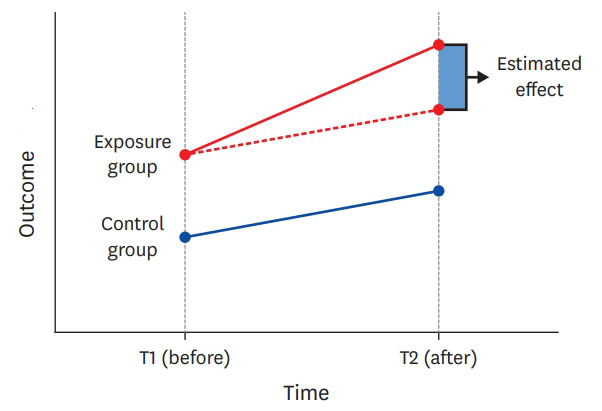
\includegraphics[width=\textwidth]{../../LaTex/img/DiD.png}    
        \end{center}
    \end{minipage}   
    
    
\end{frame}

\begin{frame}{DiD estimator. Advantages are weaknesses}
    
\begin{itemize}
    \item \textbf{Advantage:} Accounts for external time-varying confounders, as long as they affect treatment and control groups equally over time.
    \item \textbf{Weakness:} Biased estimation if the time-dependency of the confounders differs between the control and treatment group.
\end{itemize}

\end{frame}

\begin{frame}{DiD estimator. An Example}

    \textbf{Example:} A study evaluates the impact of a new transportation subsidy on student attendance:
    \begin{itemize}
        \item \textbf{Data:} Attendance rates are measured for both students in districts with and without the subsidy before and after its introduction.
        \item \textbf{Causal effect estimate:} Before-and-after estimate minus the difference in the outcome for control group after and before the treatment
        \item \textbf{Assumption of Parallel Trends:}
        \begin{itemize}
            \item[$\bullet$] \textbf{Met:} Factors like economic conditions, weather, or school policies influence attendance similarly in both districts over time.
            \item[$\bullet$] \textbf{Not Met:} If one district experiences an unrelated policy change (e.g., stricter truancy enforcement) or a unique event (e.g., a school closure due to weather).
        \end{itemize}
    \end{itemize}
    
\end{frame}

\begin{frame}{DiD estimator}

\begin{coolblock}{DiD estimator}
    The DiD estimator is defined as
    $$
    \widehat{\mathrm{SATE}}_{DiD} 
    = \underbrace{(\oline{Y}_T^{\mathrm{after}} - \oline{Y}_T^{\mathrm{before}})}_{\parbox{3.25cm}{\text{\tiny difference for the treatment group} \\ [-0.1cm] {\tiny $ = \widehat{SATE}_{BA}$}}}  - \underbrace{(\oline{Y}_C^{\mathrm{after}} - \oline{Y}_C^{\mathrm{before}})}_{\text{\tiny difference for the control group}},
    $$ 
    where $\oline{Y}_T^{\mathrm{after}}$ and $\oline{Y}_T^{\mathrm{before}}$ refers to the pre and posttreatment sample average of the outcome in the treatment group, while $\oline{Y}_C^{\mathrm{after}}$ and $\oline{Y}_C^{\mathrm{before}}$ hold analogous definitions for the control group.
\end{coolblock}
    
\end{frame}

\end{document}
